\documentclass{article}
% Chinese Support using xeCJK
% \usepackage{xeCJK}
% \setCJKmainfont{SimSun}

% Chinese Support using CTeX
\usepackage{ctex}

% Math Support
\usepackage{amsmath}
\usepackage{amsfonts}
\usepackage{amssymb}
\usepackage{wasysym}
\newcommand{\angstrom}{\text{\normalfont\AA}}

\usepackage{fancyhdr}

% Graphics Support
\usepackage{graphicx}
\usepackage{float}

% Reduced page margin
\usepackage{geometry}
\geometry{a4paper,scale=0.8}

\usepackage{caption}
\usepackage{subcaption}

% d and e should be math operators
\newcommand*{\dif}{\mathop{}\!\mathrm{d}}
\newcommand*{\md}{\mathop{}\!\mathrm{d}}
\newcommand*{\me}{\mathrm{e}}
\newcommand*{\mh}{\mathrm{h}}
\newcommand*{\Jmath}{J}

% No indent for each paragraph
\usepackage{parskip}
\setlength{\parindent}{0cm}

% Bold style for Greek letters
\usepackage{bm}
\let\Oldmathbf\mathbf
\renewcommand{\mathbf}[1]{\boldsymbol{\Oldmathbf{#1}}}

% More space for dfrac in cell
\usepackage{cellspace}
\setlength{\cellspacetoplimit}{5pt}
\setlength{\cellspacebottomlimit}{5pt}

% SI units
\newcommand{\si}[1]{\  \mathrm{#1}}

% Multi-line author information
\usepackage{authblk}
\author{物理(4+4)1801 \quad 胡喜平 \quad 学号 U201811966}

\affil{网站 https://hxp.plus/ \quad 邮件 hxp201406@gmail.com}

\title{《量子力学教程》课后习题——第二章\ 波函数和薛定谔方程}

\pagestyle{fancy}
\fancyhf{}
\lhead{源码地址:https://github.com/hxp-plus/Notes/blob/master/Qumntum-Mechenics/Homework/}
\rfoot{第 \thepage 页}
\renewcommand{\headrulewidth}{1pt}
\renewcommand{\footrulewidth}{1pt}

\usepackage{pdfpages}

\begin{document}

\maketitle\thispagestyle{fancy}

\paragraph{2.1}

证明在定态中,概率流密度与时间无关。

\paragraph{解}

定态波函数为

\begin{equation*}
  \begin{aligned}
    \psi \left( r,t \right) = \psi \left( r \right) \exp \left[ - \dfrac{i E}{\hbar} t  \right]
  \end{aligned}
\end{equation*}

概率流密度为

\begin{equation*}
  \begin{aligned}
    J &= \dfrac{\hbar}{2i \mu} \left| \psi \left( r \right) \right|^2 \nabla \ln \left\{ \dfrac{\psi \left( r \right)}{\psi^{*} \left( r \right)} \exp \left[ - \dfrac{2 i E}{\hbar}t  \right]  \right\}
    =\dfrac{\hbar}{2i\mu} \left| \psi \left( r \right) \right|^2 \nabla \left\{ \ln \left[ \dfrac{\psi \left( r \right)}{\psi^{*} \left( r \right)}  \right] + \dfrac{2iEt}{\hbar}  \right\} \\
    &= \dfrac{\hbar}{2i\mu} \left| \psi \left( r \right) \right|^2 \nabla \ln \left[ \dfrac{\psi \left( r \right)}{\psi^{*} \left( r \right)}  \right]
  \end{aligned}
\end{equation*}

与时间无关。

\paragraph{2.2}

由下列两定态波函数计算概率流密度。

\begin{equation*}
  \begin{aligned}
    \psi_1 = \dfrac{1}{r} \exp \left[ i k r \right]
    \quad\quad \quad\quad \quad\quad 
    \psi_2 = \dfrac{1}{r} \exp \left[ - i k r \right] 
  \end{aligned}
\end{equation*}

从所得结果说明$\psi_1$表示向外传播的球面波,$\psi_2$表示向内(即向原点)传播的球面波。

\paragraph{解}

\begin{equation*}
  \begin{aligned}
    \vec{\Jmath}_1 = \dfrac{\hbar}{2 i \mu} \left| \psi \right|^2  \nabla \ln \dfrac{\psi}{\psi^{*}} = \dfrac{\hbar}{2i\mu} \dfrac{1}{r^2} \nabla \left( 2ikr \right) = \dfrac{\hbar k}{\mu r^2} \vec{e}_r 
  \end{aligned}
\end{equation*}

\begin{equation*}
  \begin{aligned}
    \vec{\Jmath}_2 = \dfrac{\hbar}{2 i \mu} \left| \psi \right|^2  \nabla \ln \dfrac{\psi}{\psi^{*}} = \dfrac{\hbar}{2i\mu} \dfrac{1}{r^2} \nabla \left( -2ikr \right) = - \dfrac{\hbar k}{\mu r^2} \vec{e}_r 
  \end{aligned}
\end{equation*}

$\psi_1$是沿着$\vec{e}_r$方向传播的,$\psi_2$是沿着$\vec{e}_r$相反方向传播的。

\paragraph{2.3}

一粒子在一维势场

\begin{equation*}
  \begin{aligned}
    U \left( x \right) =
  \end{aligned}
  \left\{
  \begin{aligned}
    & \infty && x<0 \\
    & 0 && 0 \leq x \leq a \\
    & \infty && x>a
  \end{aligned}
  \right.
\end{equation*}

中运动,求粒子的能级和对应的波函数。

\paragraph{解}

在$0<x<a$时,薛定谔方程

\begin{equation*}
  \begin{aligned}
    - \dfrac{\hbar^2}{2\mu} \dfrac{\md^2 \psi}{\md x^2} = E \psi  
  \end{aligned}
\end{equation*}

即

\begin{equation*}
  \begin{aligned}
    \dfrac{\md^2 \psi}{\md x^2} - \dfrac{\hbar^2}{2 \mu E} \psi = 0  
  \end{aligned}
\end{equation*}

设

\begin{equation*}
  \begin{aligned}
    \psi = A \cos \alpha x + B \sin \alpha x
  \end{aligned}
\end{equation*}

代入解得

\begin{equation*}
  \begin{aligned}
    \psi = A \cos \alpha x + B \sin \alpha x
    \quad\quad
    \quad\quad
    \alpha = \sqrt{\dfrac{2 \mu E}{\hbar^2} }
  \end{aligned}
\end{equation*}

由波函数连续条件

\begin{equation*}
  \begin{aligned}
    \psi|_{x=0} = \psi|_{x=a} = 0
  \end{aligned}
\end{equation*}

得到

\begin{equation*}
  \begin{aligned}
    A=0
    \quad\quad
    \quad\quad
    B \sin \alpha a = 0
    \Rightarrow
    \sqrt{\dfrac{2 \mu E}{\hbar^2} } = \alpha = \dfrac{n\pi}{a} 
    \Rightarrow
    E_n = \dfrac{\pi^2 \hbar^2}{2 \mu a^2} n^2 
  \end{aligned}
\end{equation*}

由波函数归一化条件

\begin{equation*}
  \begin{aligned}
    \int_0^a \left[ B \sin \dfrac{n \pi}{a} x  \right]^2 \md x
    = B^2 \int_0^a \dfrac{1 - \cos \dfrac{2n\pi}{a}x}{2} \md x
    = \dfrac{B^2}{2} a = 1 
  \end{aligned}
\end{equation*}

解得

\begin{equation*}
  \begin{aligned}
    B = \sqrt{\dfrac{2}{a} } 
  \end{aligned}
\end{equation*}

因此波函数为

\begin{equation*}
  \begin{aligned}
    \psi_n \left( x \right) = 
  \end{aligned}
  \left\{
  \begin{aligned}
    & \sqrt{\dfrac{2}{a}  } \sin \dfrac{n \pi}{a}x && 0< x < a \\
    & 0 && x<0,x>a
  \end{aligned}
  \right.
\end{equation*}






\paragraph{2.4}

证明下式中的归一化因子是$A'=\dfrac{1}{\sqrt{a}} $

\begin{equation*}
  \begin{aligned}
    \psi_n =
  \end{aligned}
  \left\{
  \begin{aligned}
    & A' \sin \dfrac{n\pi}{2a} \left( x + a \right) && \left| x \right| < a \\
    & 0 && \left| x \right| \geq a
  \end{aligned}
  \right.
\end{equation*}

\paragraph{解}

\begin{equation*}
  \begin{aligned}
    \int_{-a}^a \left[ A' \sin \dfrac{n\pi}{a} \left( x + a \right)  \right]^2 \md x
    = \dfrac{A'^2}{2} \int_{-a}^a \left[ 1 - \cos \dfrac{2n\pi}{a} \left( x +a \right)  \right] \md x
    = A'^2 a = 1
    \Rightarrow
    A' = \dfrac{1}{\sqrt{a}} 
  \end{aligned}
\end{equation*}

\paragraph{2.5}

求一维谐振子处在第一激发态时概率最大的位置。

\paragraph{解}

对应能量$E_n$的波函数是

\begin{equation*}
  \begin{aligned}
    \psi_n \left( \xi \right)
    = N_n \exp \left[ - \dfrac{\xi^2}{2}  \right] H_n \left( \xi \right)
    \quad\quad
    \xi = \alpha x
    \quad\quad
    N_n
    = \left( \dfrac{\alpha}{\pi^{\frac{1}{2} } 2^n n!}  \right)^{\frac{1}{2} }
  \end{aligned}
\end{equation*}

$n=1$时

\begin{equation*}
  \begin{aligned}
    \psi_1 \left( x \right)
    = \left( \dfrac{\alpha}{2\sqrt{\pi}}  \right)^{\frac{1}{2}} \exp \left[ - \dfrac{\alpha^2}{2} x^2  \right] \cdot 2\alpha x
  \end{aligned}
\end{equation*}

概率为

\begin{equation*}
  \begin{aligned}
    w \left( x \right)
    = \left| \psi \left( x \right) \right|^2
    = \dfrac{2 \alpha^3}{\sqrt{\pi}} x^2 \exp \left[ - \alpha^2 x^2 \right]
  \end{aligned}
\end{equation*}

对概率求导数

\begin{equation*}
  \begin{aligned}
    \dfrac{\md w \left( x \right)}{\md x}
    = \dfrac{4 \alpha^3}{\sqrt{\pi}} \left[ x \left( 1 - \alpha^2 x^2 \right) \right] \exp \left[ -a^2 x^2 \right]
  \end{aligned}
\end{equation*}

\begin{equation*}
  \begin{aligned}
    \dfrac{\md^2 w \left( x \right)}{\md x^2}
    = \dfrac{4\alpha^3}{\sqrt{\pi}} \left( 2 \alpha^4 - 5 \alpha^2 x^2 + 1 \right) \exp \left[ - \alpha^2 x^2 \right]
  \end{aligned}
\end{equation*}

只有当$x=\pm \dfrac{1}{\alpha} $时,$\dfrac{\md w \left( x \right)}{\md x} = 0$且$\dfrac{\md^2 w \left( x \right)}{\md x^2} < 0 $,因此最大概率位置$x=\pm \dfrac{1}{\alpha} $

\paragraph{2.6}

在一维势场中运动的粒子,势能对原点对称:$U \left( - x \right) = U \left( x \right)$,证明粒子的定态波函数具有确定的宇称。

\paragraph{解}

薛定谔方程为

\begin{equation*}
  \begin{aligned}
    \dfrac{\md^2 \psi \left( x \right)}{\md x^2} + \dfrac{2 \mu}{\hbar^2} \left[ E - U \left( x \right) \right] \psi \left( x \right) = 0  
  \end{aligned}
\end{equation*}

\begin{equation*}
  \begin{aligned}
    \dfrac{\md^2 \psi \left( -x \right)}{\md x^2} + \dfrac{2 \mu}{\hbar^2} \left[ E - U \left( x \right) \right] \psi \left( -x \right) = 0  
  \end{aligned}
\end{equation*}

$\psi \left( x \right)$和$\psi \left( -x \right)$是一个方程的解,它们的线性组合也是方程的解。因此下面两个方程是薛定谔方程的解

\begin{equation*}
  \begin{aligned}
    \psi_e \left( x \right) = \psi \left( x \right) + \psi \left( -x \right)
  \end{aligned}
\end{equation*}

\begin{equation*}
  \begin{aligned}
    \psi_o \left( x \right) = \psi \left( x \right) - \psi \left( -x \right)
  \end{aligned}
\end{equation*}

其中$\psi_e \left( x \right)$是偶函数,$\psi_o \left( x \right)$是奇函数。因此有确定的宇称。

\paragraph{2.7}

一粒子在一维深势阱

\begin{equation*}
  \begin{aligned}
    U \left( x \right) =
  \end{aligned}
  \left\{
  \begin{aligned}
    & V_0 > 0 && \left| x \right| > a \\
    & 0 && \left| x \right| \leq a
  \end{aligned}
  \right.
\end{equation*}

中运动,求束缚态($0<E<V_0$)的能级所满足的方程。

\paragraph{解}

(这个方法参考了附在后面的文档,文档节选自David A.B. Miller的Quantum Mechanics,我觉得这个方法比较有意思就研究了下)

设波函数的解为

\begin{equation*}
  \begin{aligned}
    \psi \left( x \right) =
  \end{aligned}
  \left\{
  \begin{aligned}
    & G \exp \left( \kappa x \right) && x<-a \\
    & A \sin kx + B \cos kx && -a < x < a \\
    & F \exp \left( - \kappa x \right)
  \end{aligned}
  \right.
\end{equation*}

其中

\begin{equation*}
  \begin{aligned}
    & \kappa = \sqrt{2m \left( V_0 - E \right) / \hbar^2} \\
    & k = \sqrt{2mE / \hbar^2}
  \end{aligned}
\end{equation*}

设

\begin{equation*}
  \begin{aligned}
    X_L &= \exp \left( - \kappa a \right) \\
    S_L &= \sin \left( k a \right) \\
    C_L &= \cos \left( k a \right)
  \end{aligned}
\end{equation*}

连续性给出

\begin{equation*}
  \begin{aligned}
    G X_L &= - AS_L + BC_L \\
    F X_L &= A S_L + BC_L \\
    \dfrac{\kappa}{k} GX_L &= AC_L + BS_L \\
    - \dfrac{\kappa}{k} FX_L &= AC_L - BS_L
  \end{aligned}
\end{equation*}

解出

\begin{equation*}
  \begin{aligned}
    2BC_L &= \left( F + G \right) X_L \\
    2BS_L &= \dfrac{\kappa}{k} \left( F + G \right) X_L 
  \end{aligned}
\end{equation*}

有两组解

\begin{equation*}
  \begin{aligned}
    \tan ka &= \dfrac{\kappa}{k} && F\neq -G \\
    -\cot ka &= \dfrac{\kappa}{k} && F \neq G 
  \end{aligned}
\end{equation*}

其中$F= G$和$F= -G$必须满足一个,否则无解。定义

\begin{equation*}
  \begin{aligned}
    E_1^{\infty} &= \dfrac{\hbar^2}{2m} \left( \dfrac{2\pi}{a}  \right)^2 \\
    \varepsilon &= \dfrac{E}{E_1^{\infty}} \\
    v_0 &= \dfrac{V_0}{E_1^{\infty}} 
  \end{aligned}
\end{equation*}

则

\begin{equation*}
  \begin{aligned}
    \dfrac{\kappa}{k} &= \sqrt{\dfrac{v_0 - \varepsilon}{\varepsilon} } \\
    k a &= \dfrac{\pi}{2} \sqrt{\dfrac{E}{E_1^{\infty}} } = \dfrac{\pi}{2} \sqrt{\varepsilon}  \\
    \kappa a &= \dfrac{\pi}{2} \sqrt{\dfrac{V_0 - E}{E_1^{\infty}} } = \dfrac{\pi}{2} \sqrt{v_0 - \varepsilon}  
  \end{aligned}
\end{equation*}

定义

\begin{equation*}
  \begin{aligned}
    c_L &= \dfrac{C_L}{X_L} = \dfrac{\cos \left( \pi \sqrt{\varepsilon} / 2 \right)}{\exp \left( - \pi \sqrt{v_0 - \varepsilon} / 2 \right)} \\
    s_L &= \dfrac{S_L}{X_L} = \dfrac{\sin \left( \pi \sqrt{\varepsilon} / 2 \right)}{\exp \left(  - \pi \sqrt{v_0 - \varepsilon}/2 \right)}  
  \end{aligned}
\end{equation*}

当$F=G$时

\begin{equation*}
  \begin{aligned}
    \sqrt{\varepsilon} \tan \left( \dfrac{\pi}{2} \sqrt{\varepsilon}  \right) = \sqrt{v_0 - \varepsilon}
  \end{aligned}
\end{equation*}

波函数为

\begin{equation*}
  \begin{aligned}
    \psi \left( x \right) = 
  \end{aligned}
  \left\{
  \begin{aligned}
    & B c_L \exp \left(2 \pi \sqrt{v_0 - \varepsilon} \cdot \dfrac{x}{a}  \right) \\
    & B \cos \left( 2 \pi \sqrt{\varepsilon} \cdot \dfrac{x}{a}  \right) \\
    & B c_L \exp \left( - 2 \pi \sqrt{v_0 - \varepsilon} \cdot \dfrac{x}{a}  \right)
  \end{aligned}
  \right.
\end{equation*}

当$F=-G$时

\begin{equation*}
  \begin{aligned}
    - \sqrt{\varepsilon} \cot \left( \dfrac{\pi}{2} \sqrt{\varepsilon}  \right) = \sqrt{v_0 - \varepsilon}
  \end{aligned}
\end{equation*}

波函数为

\begin{equation*}
  \begin{aligned}
    \psi \left( x \right) = 
  \end{aligned}
  \left\{
  \begin{aligned}
    & - A s_L \exp \left(2 \pi \sqrt{v_0 - \varepsilon} \cdot \dfrac{x}{a}  \right) \\
    & A \sin \left( 2 \pi \sqrt{\varepsilon} \cdot \dfrac{x}{a}  \right) \\
    & A s_L \exp \left( - 2 \pi \sqrt{v_0 - \varepsilon} \cdot \dfrac{x}{a}  \right)
  \end{aligned}
  \right.
\end{equation*}

\paragraph{2.8}

分子间的范德瓦尔斯力所产生的势能可以近似地表示为

\begin{equation*}
  \begin{aligned}
    U \left( x  \right) = 
  \end{aligned}
  \left\{
  \begin{aligned}
    & \infty && x<0 \\
    & U_0 && 0 \leq x < a \\
    & - U_1 && a \leq x \leq b \\
    & 0 && b < x
  \end{aligned}
  \right.
\end{equation*}

求束缚态的能级所满足的方程。

\paragraph{解}

设波函数的解为

\begin{equation*}
  \begin{aligned}
    \psi \left( x \right) =
  \end{aligned}
  \left\{
  \begin{aligned}
    & 0 && x<0 \\
    & A \exp \left( \kappa_0 x \right) - A \exp \left( - \kappa_0 x \right) && 0<x<a \\
    & C \sin kx + D \cos kx && a<x<b \\
    & G \exp \left( - \kappa_2 x \right) && x>b
  \end{aligned}
  \right.
\end{equation*}

其中

\begin{equation*}
  \begin{aligned}
    \kappa_0 &= \sqrt{2 m \left( U_0 - E \right) / \hbar^2} \\
    k &= \sqrt{ 2m \left( U_1 + E \right) / \hbar^2 } \\
    \kappa_2 &= \sqrt{-2mE/ \hbar^2}
  \end{aligned}
\end{equation*}

波函数边界连续条件给出

\begin{equation*}
  \begin{aligned}
    & A \exp \left( \kappa_0 a \right) - A \exp \left( - \kappa_0 a \right) = C \sin ka + D \cos ka \\
    & \kappa_0 A \exp \left( \kappa_0 a \right) + \kappa_0 A = kC \cos ka - kD \sin ka \\
    & G \exp \left(  - \kappa_2 b \right) = C \sin kb - D \cos kb \\
    & - \kappa_2 G \exp \left( - \kappa_2 b \right) = k C \cos kb - kD \sin kb
  \end{aligned}
\end{equation*}

即

\begin{equation*}
  \begin{aligned}
    \left[
      \begin{array}{cccc}
       2\sinh \kappa_0 a & -\sin ka & -\cos ka & 0 \\
       2\kappa_0 \cosh \kappa_0 a & - k \cos ka & k\sin ka & 0 \\
       0 & - \sin kb & -\cos kb & \exp \left( - \kappa_2 b \right) \\
       0 & - k \cos kb & k \sin kb & - \kappa_2 \exp \left( - \kappa_2 b \right)
      \end{array}
    \right ]
  \end{aligned}
  \begin{aligned}
    \left[
      \begin{array}{c}
       A \\
       C \\
       D \\
       G 
      \end{array}
    \right ]
    =0 
  \end{aligned}
\end{equation*}

波函数有解的条件是

\begin{equation*}
  \begin{aligned}
    \left|
      \begin{array}{cccc}
       2\sinh \kappa_0 a & -\sin ka & -\cos ka & 0 \\
       2\kappa_0 \cosh \kappa_0 a & - k \cos ka & k\sin ka & 0 \\
       0 & - \sin kb & -\cos kb & \exp \left( - \kappa_2 b \right) \\
       0 & - k \cos kb & k \sin kb & - \kappa_2 \exp \left( - \kappa_2 b \right)
      \end{array}
    \right|
  \end{aligned}
\end{equation*}

即能量需满足关系

\begin{equation*}
  \begin{aligned}
    \tan k \left( b - a \right) = \dfrac{k \kappa_0 \coth \kappa_0 a + k \kappa_2}{k^2 - \kappa_0 \kappa_2 \coth \kappa_0 a} 
  \end{aligned}
\end{equation*}

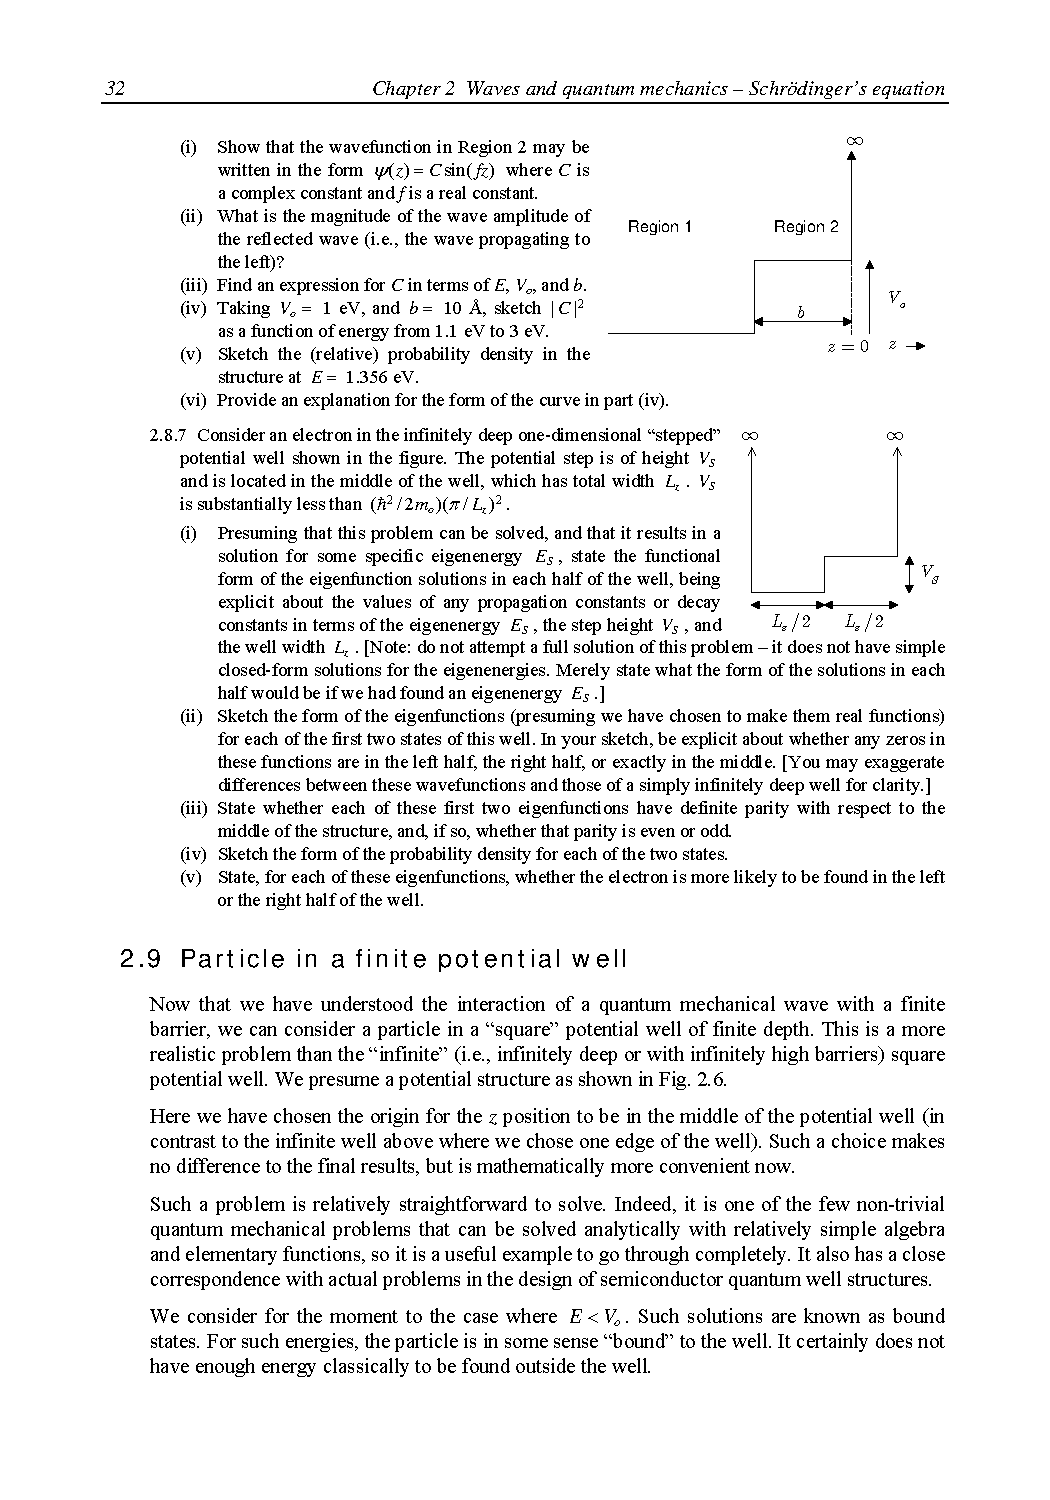
\includepdf[pages={1-4},angle=0]{量子力学作业2-7不用行列式的解法.pdf}

\end{document} 
